\documentclass[noauthor,nooutcomes,handout]{ximera}

\graphicspath{  
{./}
{./whoAreYou/}
{./drawingWithTheTurtle/}
{./bisectionMethod/}
{./circles/}
{./anglesAndRightTriangles/}
{./lawOfSines/}
{./lawOfCosines/}
{./plotter/}
{./staircases/}
{./pitch/}
{./qualityControl/}
{./symmetry/}
{./nGonBlock/}
}


%% page layout
\usepackage[cm,headings]{fullpage}
\raggedright
\setlength\headheight{13.6pt}


%% fonts
\usepackage{euler}

\usepackage{FiraMono}
\renewcommand\familydefault{\ttdefault} 
\usepackage[defaultmathsizes]{mathastext}
\usepackage[htt]{hyphenat}

\usepackage[T1]{fontenc}
\usepackage[scaled=1]{FiraSans}

%\usepackage{wedn}
\usepackage{pbsi} %% Answer font


\usepackage{cancel} %% strike through in pitch/pitch.tex


%% \usepackage{ulem} %% 
%% \renewcommand{\ULthickness}{2pt}% changes underline thickness

\tikzset{>=stealth}

\usepackage{adjustbox}

\setcounter{titlenumber}{-1}

%% journal style
\makeatletter
\newcommand\journalstyle{%
  \def\activitystyle{activity-chapter}
  \def\maketitle{%
    \addtocounter{titlenumber}{1}%
                {\flushleft\small\sffamily\bfseries\@pretitle\par\vspace{-1.5em}}%
                {\flushleft\LARGE\sffamily\bfseries\thetitlenumber\hspace{1em}\@title \par }%
                {\vskip .6em\noindent\textit\theabstract\setcounter{question}{0}\setcounter{sectiontitlenumber}{0}}%
                    \par\vspace{2em}
                    \phantomsection\addcontentsline{toc}{section}{\thetitlenumber\hspace{1em}\textbf{\@title}}%
                     }}
\makeatother



%% thm like environments
\let\question\relax
\let\endquestion\relax

\newtheoremstyle{QuestionStyle}{\topsep}{\topsep}%%% space between body and thm
		{}                      %%% Thm body font
		{}                              %%% Indent amount (empty = no indent)
		{\bfseries}            %%% Thm head font
		{)}                              %%% Punctuation after thm head
		{ }                           %%% Space after thm head
		{\thmnumber{#2}\thmnote{ \bfseries(#3)}}%%% Thm head spec
\theoremstyle{QuestionStyle}
\newtheorem{question}{}



\let\freeResponse\relax
\let\endfreeResponse\relax

%% \newtheoremstyle{ResponseStyle}{\topsep}{\topsep}%%% space between body and thm
%% 		{\wedn\bfseries}                      %%% Thm body font
%% 		{}                              %%% Indent amount (empty = no indent)
%% 		{\wedn\bfseries}            %%% Thm head font
%% 		{}                              %%% Punctuation after thm head
%% 		{3ex}                           %%% Space after thm head
%% 		{\underline{\underline{\thmname{#1}}}}%%% Thm head spec
%% \theoremstyle{ResponseStyle}

\usepackage[tikz]{mdframed}
\mdfdefinestyle{ResponseStyle}{leftmargin=1cm,linecolor=black,roundcorner=5pt,
, font=\bsifamily,}%font=\wedn\bfseries\upshape,}


\ifhandout
\NewEnviron{freeResponse}{}
\else
%\newtheorem{freeResponse}{Response:}
\newenvironment{freeResponse}{\begin{mdframed}[style=ResponseStyle]}{\end{mdframed}}
\fi



%% attempting to automate outcomes.

%% \newwrite\outcomefile
%%   \immediate\openout\outcomefile=\jobname.oc
%% \renewcommand{\outcome}[1]{\edef\theoutcomes{\theoutcomes #1~}%
%% \immediate\write\outcomefile{\unexpanded{\outcome}{#1}}}

%% \newcommand{\outcomelist}{\begin{itemize}\theoutcomes\end{itemize}}

%% \NewEnviron{listOutcomes}{\small\sffamily
%% After answering the following questions, students should be able to:
%% \begin{itemize}
%% \BODY
%% \end{itemize}
%% }
\usepackage[tikz]{mdframed}
\mdfdefinestyle{OutcomeStyle}{leftmargin=2cm,rightmargin=2cm,linecolor=black,roundcorner=5pt,
, font=\small\sffamily,}%font=\wedn\bfseries\upshape,}
\newenvironment{listOutcomes}{\begin{mdframed}[style=OutcomeStyle]After answering the following questions, students should be able to:\begin{itemize}}{\end{itemize}\end{mdframed}}



%% my commands

\newcommand{\snap}{{\bfseries\itshape\textsf{Snap!}}}
\newcommand{\flavor}{\link[\snap]{https://snap.berkeley.edu/}}
\newcommand{\mooculus}{\textsf{\textbf{MOOC}\textnormal{\textsf{ULUS}}}}


\usepackage{tkz-euclide}
\tikzstyle geometryDiagrams=[rounded corners=.5pt,ultra thick,color=black]
\colorlet{penColor}{black} % Color of a curve in a plot



\ifhandout\newcommand{\mynewpage}{\newpage}\else\newcommand{\mynewpage}{}\fi


\title{Angles and right triangles}
\author{Bart Snapp}

\begin{document}
\begin{abstract}
  We learn about Pythagorean triples.
\end{abstract}
\maketitle

\begin{listOutcomes}
\item{Understand what Pythagorean triples are.}
\item{Know how to identify Pythagorean triples.}
\item{Use \snap\ to draw right triangles, given a Pythagorean triple.}
\item{Apply the bisection method to solve a problem where no equation is given.}
\item{Describe the bisection method as an algorithm.}
\end{listOutcomes}
\begin{listObjectives}
 \item Learn and apply basic geometric formulas,
\item Explain why presented concepts and formulas are true,
\item Use trigonometry to solve common problems.
\end{listObjectives}

\begin{question}
 Using what you know about sine, cosine, and right triangles, draw and label a right triangle where $\cos(\theta)=\frac{3}{5}$, then find $\sin(\theta)$.
\end{question}
\mynewpage

\begin{question}
  Now imagine a right triangle with a hypotenuse of length $1$. 
  \begin{enumerate}
  \item For a given nonright angle of the triangle, call it $\theta$,
    Explain why one leg of the triangle has length $\cos(\theta)$ and
    the other has length $\sin(\theta)$.  Use words, pictures, and so
    on, as needed/helpful in your explanation.
  \item Explain why
    \[
    \cos^2(\theta) + \sin^2(\theta) = 1.
    \]
  \item Use your work above to Explain why
    \[
    (x,y) = (\sin(\theta),\cos(\theta))
    \]
    will always lie on a unit circle centered at the origin for any
    angle $\theta$.
  \end{enumerate}
  \begin{freeResponse}
    \begin{enumerate}
    \item Given a right triangle
    \begin{center}
      \begin{tikzpicture}[geometryDiagrams]
        \coordinate (A) at (0,0);
        \coordinate (B) at (0,3);
        \coordinate (C) at (7,0);
        \tkzDrawSegment (A,B)
        \tkzDrawSegment (A,C)
        \tkzDrawSegment (C,B)
        \tkzLabelSegment[left](A,B){$a$}
        \tkzLabelSegment[below](A,C){$b$}
        \tkzLabelSegment[above right](B,C){$1$}  

        \tkzMarkRightAngle[thin](C,A,B)
        %\tkzLabelAngle[pos=1.2](C,A,B){$?$}

        %\tkzMarkAngle[size=0.8cm,thin,mark=](A,B,C)
        %\tkzLabelAngle[pos=.5](A,B,C){$\beta$}

        \tkzMarkAngle[mark=,size=1.2cm,thin](B,C,A)
        \tkzLabelAngle[pos=.9](B,C,A){$\theta$}
      \end{tikzpicture}
    \end{center}
    We see
    \[
    \sin(\theta) = \frac{a}{1} = a\qquad \text{and}\qquad \cos(\theta) = \frac{b}{1} = b.
    \]
  \item With the same right triangle above, we also see via the Pythagorean theorem:
    \[
    \cos^2(\theta) + \sin^2(\theta) = 1.
    \]
  \item Since
    \[
    x^2+y^2=1
    \]
    is the set of points making a unit circle and
    \[
    \sin^2(\theta) + \cos^2(\theta) = 1
    \]
    we see that $x=\sin(\theta)$ and $y=\cos(\theta)$ will always be
    on the circle.
    \end{enumerate}
  \end{freeResponse}
\end{question}
\mynewpage

\begin{question}
  Let's think about our previous work a little more.
  \begin{enumerate}
  \item Consider the following \snap\ block \raisebox{-.4\height}{
\includegraphics{../sineAndCosine/circleBlank.png}}. Here is the script for that block:
    \begin{center}
      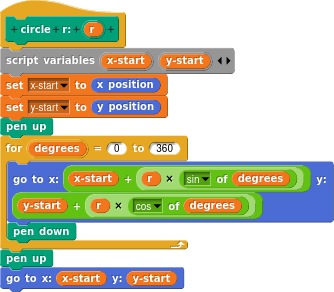
\includegraphics{../sineAndCosine/circleScript.png}
    \end{center}
    Explain how the script works, block-by-block as you would like to
    have it explained to you. Use words, pictures, and so on, as
    needed/helpful in your explanation.
  \item Some folks like to plot circles with:
    \[
    (x,y) = (\cos(\theta),\sin(\theta)) \qquad\text{others with}\qquad  (x,y) = (\sin(\theta),\cos(\theta))
    \]
    How does the command \raisebox{-.4\height}{
\includegraphics{../sineAndCosine/circleBlank.png}} change if you change how it plots circles?
%  \item Find real world circumstances where it might be better to use $(x,y) = (\sin(\theta),\cos(\theta))$. Explain your reasoning.
%  \item Find real world circumstances where it might be better to use $(x,y) = (\cos(\theta),\sin(\theta))$. Explain your reasoning.
  
  \end{enumerate}
  \begin{freeResponse}
    \begin{enumerate}
    \item Here we go:
      \begin{enumerate}
      \item The user tells us the radius $r$.
      \item We have variables \texttt{x-start} and \texttt{y-start}
        and we set them to the current position of the turtle.
      \item Next we pick up the pen and move to the first point on the circle.
      \item Now for each degree, we move to another point on the circle, $x= \texttt{x-start} + \sin(\theta)$. $y= \texttt{y-start} + \cos(\theta)$. 
      \item Finally, we pick up the pen and return to where we started.
      \end{enumerate}
    \item As written, the command starts drawing the circle at the top
      and travels in a clockwise direction. If we swap sine and
      cosine, then it will start at the right and travel in a
      counterclockwise direction.
    \item So it would be better to use $(x,y) =
      (\sin(\theta),\cos(\theta))$ when modeling a clock, as a clock starts at the top and travels clockwise.
    \item It would be better to use $(x,y) =
      (\cos(\theta),\sin(\theta))$ when modeling latitude, as the
      equator is at zero degrees, then we travel up to the pole at
      $90$ degrees.
    \end{enumerate}
  \end{freeResponse}
\end{question}
\mynewpage

%\begin{question}
%Explain what a Pythagorean triple is as you would like to have them
%  explained to you. In particular, as part of this explanation:
%  \begin{enumerate}
%    \item Explain what a \textbf{primitive} Pythagorean triple is.
%    \item Give $3$ examples of nonprimitive Pythagorean triples and
%      $3$ more examples of primitive Pythagorean triples.
%    \item Someone once said, ``every Pythagorean triple is
%      \textbf{similar} to a primitive Pythagorean triple.'' Explain
%      what this means.
%  \end{enumerate}
%  \begin{freeResponse}
%    A \underline{Pythagorean triple} is a list of three whole numbers
%    $(a,b,c)$ where if $c$ is the largest such number,
%    \[
%    a^2 + b^2 = c^2.
%    \]
%    This means, from our previous work, that there is a right triangle
%    with these whole number side lengths.
%    \begin{enumerate}
%    \item A Pythagorean triple $(a,b,c)$ is called \underline{primitive} if
%    none of $a$, $b$, or $c$ have a common whole number factor other
%    than $1$.
%    \item If a Pythagorean triple $(a,b,c)$ is nonprimitive if $a$,
%      $b$, and $c$ have a whole number common factor bigger than
%      $1$. So
%    \[
%    (6,8,10), \qquad (10,24,26), \qquad (16,30,34), 
%    \]
%    are all nonprimitive Pythagorean triples. If we divide by the
%    common factors, we get the following primitive Pythagorean
%    triples
%    \[
%    (3,4,5), \qquad (5,12,13), \qquad (8,15,17).
%    \]
%
%  \item Triangles are \underline{similar} if the sides of one are a scalar
%    multiple of the sides of another. So we see every nonprimitive
%    Pythagorean triple is indeed similar to a primitive Pythagorean
%    triple.
%    \end{enumerate}
%  \end{freeResponse}
%\end{question}
%\mynewpage
%
%\begin{question}
%  Here are $3$ Pythagorean triples:
%  \[
%  (119, 120, 169), \qquad (50,120,130), \qquad (60,80,100).
%  \]
%  In each case, make \snap\ scripts that will draw these triangles.
%     \adjustbox{valign=t}{
%    \begin{tabular}{lp{.6\textwidth}}
%      
%      \raisebox{-\height}{
%    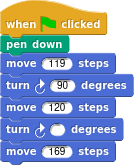
\includegraphics{basicScriptRightBlank.png}}
%
%      &
%
%      As a gesture of friendship, I'll start you off with the
%      \snap\ script on the left. You must use the \textbf{bisection
%        method} to find the angle for the final turn.  Show off your
%      WORK with a TABLE as we have done before. Demonstrate that your
%      work is correct by your by giving screenshots of your \snap\ SCRIPTS
%      and STAGES.
%     \end{tabular}}
%
%     As another gesture of friendship, I have started the three tables
%     for you. Your job is to FILL THEM IN.
%     \[
%     \begin{array}{rl}
%       \mathbf{(119,120,169):} &
%        \begin{array}{|c|c|c|c|}\hline
%       \text{Attempt} & \text{angle} & \text{Too large or too small?} \\ \hline\hline
%       1 & 130 & \text{too small} \\ \hline
%       2 & 140 & \text{too large}  \\ \hline
%       3 &  &   \\ \hline
%        \end{array} \\
%        & \\
%          \mathbf{(50,120,130):} & \begin{array}{|c|c|c|c|}\hline
%            \text{Attempt} & \text{angle} & \text{Too large or too small?} \\ \hline\hline
%            1 & 150 & \text{too small} \\ \hline
%            2 & 160 & \text{too large}  \\ \hline
%            3 &  &   \\ \hline
%            4 &  &   \\ \hline
%     \end{array} \\
%     & \\
%       \mathbf{(60,80,100):}  &
%        \begin{array}{|c|c|c|c|}\hline
%       \text{Attempt} & \text{angle} & \text{Too large or too small?} \\ \hline\hline
%       1 & 130 & \text{too small} \\ \hline
%       2 & 150 & \text{too large}  \\ \hline
%       3 &  &   \\ \hline
%       4 &  &   \\ \hline
%       5 &  &   \\ \hline
%       6 &  &   \\ \hline
%       7 &  &   \\ \hline
%        \end{array}
%     \end{array}
%     \]
%     \begin{freeResponse}
%       \begin{description}
%       \item[\underline{(119,120,169)}:] So first of all, this is a right
%        triangle as
%        \[
%        119^2 + 120^2 =169^2.
%        \]
%        We'll start with this script:
%        \begin{center}
%          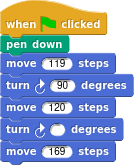
\includegraphics{basicScriptRightBlank.png}
%        \end{center}
%        If we fill in the blank with $130$ degrees, this isn't far
%        enough, if we fill it in with $140$ degrees, that is too
%        far. We're ready to do the bisection method:
%        \[
%        \begin{array}{|c|c|c|c|}\hline
%          \text{Attempt} & \text{angle} & \text{Too large or too small?} \\ \hline\hline
%          1 & 130 & \text{too small} \\ \hline
%          2 & 140 & \text{too large}  \\ \hline
%          3 & 135 & \text{BINGO!}  \\ \hline
%        \end{array}
%        \]
%        Checking the $x$-positions and $y$-positions, we have closed
%        the triangle to within $1$ unit of accuracy. Here is my script and my stage:
%        \begin{center}
%          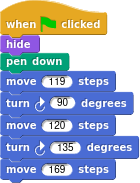
\includegraphics[width=.3\textwidth]{119120169-script.png}   \qquad \fbox{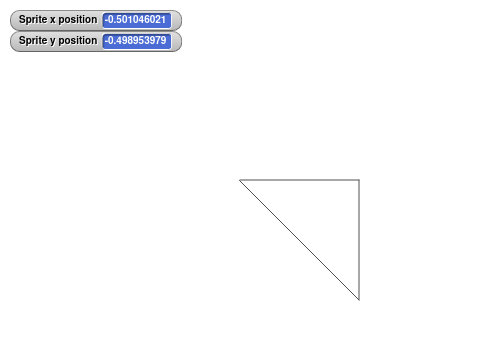
\includegraphics[width=.5\textwidth]{119120169-stage.png}}
%        \end{center}
%
%
%
%
%
%      \item[\underline{(50,120,130)}:] So first of all, this is a right
%        triangle as
%        \[
%        50^2 + 120^2 =130^2.
%        \]
%        If we fill in the blank in our script with $150$ degrees, this
%        isn't far enough, if we fill it in with $160$ degrees, that is
%        too far. We're ready to do the bisection method:
%        \[
%        \begin{array}{|c|c|c|c|}\hline
%          \text{Attempt} & \text{angle} & \text{Too large or too small?} \\ \hline\hline
%          1 & 150 & \text{too small} \\ \hline
%          2 & 160 & \text{too large}  \\ \hline
%          3 & 155 & \text{too small}  \\ \hline
%          4 & 157.5 & \text{BINGO!}  \\ \hline
%        \end{array}
%        \]
%        Checking the $x$-positions and $y$-positions, we have closed
%        the triangle to within $1$ unit of accuracy. Here is my script and my stage:
%        \begin{center}
%          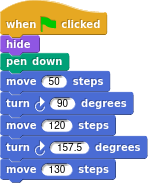
\includegraphics[width=.3\textwidth]{50120130-script.png}   \qquad \fbox{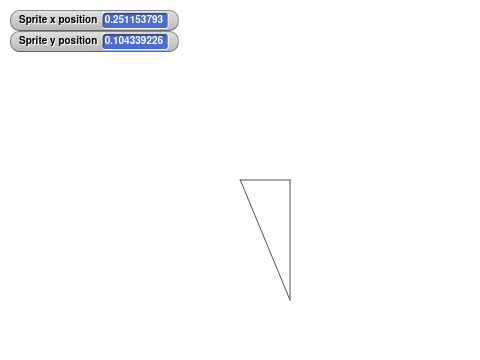
\includegraphics[width=.5\textwidth]{50120130-stage.png}}
%        \end{center}
%
%
%
%
%      
%
%
%
%      \item[\underline{(60,80,100)}:] So first of all, this is a right
%        triangle as
%        \[
%        60^2 + 80^2 = 100^2.
%        \]
%        If we fill in the blank in our script with $130$ degrees, this
%        isn't far enough, if we fill it in with $150$ degrees, that is
%        too far. We're ready to do the bisection method:
%        \[
%        \begin{array}{|c|c|c|c|}\hline
%          \text{Attempt} & \text{angle} & \text{Too large or too small?} \\ \hline\hline
%          1 & 130 & \text{too small} \\ \hline
%          2 & 150 & \text{too large}  \\ \hline
%          3 & 140 & \text{too small}  \\ \hline
%          4 & 145 & \text{too large}  \\ \hline
%          5 & 142.5 & \text{too small}  \\ \hline
%          6 & 143.75 & \text{too large}  \\ \hline
%          7 & 143.125 & \text{BINGO!}  \\ \hline
%        \end{array}
%        \]
%        Checking the $x$-positions and $y$-positions, we have closed
%        the triangle to within $1$ unit of accuracy. Here is my script and my stage:
%        \begin{center}
%          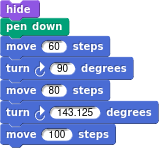
\includegraphics[width=.3\textwidth]{6080100-script.png}   \qquad \fbox{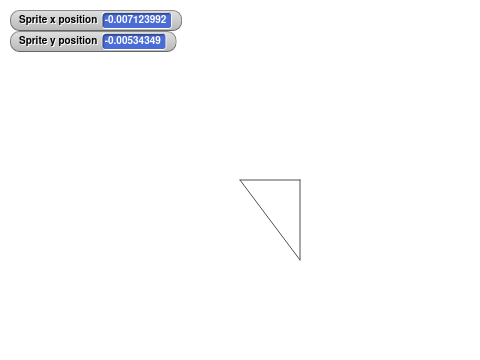
\includegraphics[width=.5\textwidth]{6080100-stage.png}}
%        \end{center}
%    \end{description}
%  \end{freeResponse}
%\end{question}
%\mynewpage
%
%
%
%\begin{question}
%  Give an algorithm for using \textbf{bisection method} to find the angles of a
%  right triangle, assuming you are given the side lengths.
%  \begin{freeResponse}
%    \begin{enumerate}
%    \item Take the shortest side, move forward this length.
%    \item Turn $90^\circ$ to the right.
%    \item Take the next longer side, move forward this length.
%    \item Now turn an \underline{unknown} number of degrees to the right.
%    \item Now move forward the longest side number of steps.
%    \item Find an angle, call it $A$ that is \underline{too large}, so
%      that the triangle's hypotenuse overlaps one of the legs.
%    \item Find an angle, call it $a$, that is \underline{too small},
%      so that that the triangle's hypotenuse doesn't meet the leg.
%    \item\label{I:stop} If $A=a$ or the hypotenuse is very close to
%      the vertex, we are done, so STOP.
%    \item Now, it must be that $A>a$. Average $A$ and $a$ and call it $m$.
%    \item Is $m$ the correct angle (or very close)? If so, then we are done, so STOP.
%    \item If $m$ is too large, change $A$ to make it equal to $m$.
%    \item If $m$ is too small, change $a$ to make it equal to $m$.
%    \item Goto step~\ref{I:stop}.
%    \end{enumerate}
%    Once you find the angle you need to turn call it $A$, we set
%    \[
%    180-\alpha = A
%    \]
%    where $\alpha$ is an interior angle of the triangle.  Hence
%    $\alpha = 180-A$. This means that the angles of the right triangle
%    are:
%    \[
%    (\alpha^\circ,90^\circ-\alpha^\circ,90^\circ).
%    \]
%  \end{freeResponse}
%\end{question}





\end{document}
